\documentclass[A4paper,]{article}
\usepackage{lmodern}
\usepackage{amssymb,amsmath}
\usepackage{ifxetex,ifluatex}
\usepackage{fixltx2e} % provides \textsubscript
\ifnum 0\ifxetex 1\fi\ifluatex 1\fi=0 % if pdftex
  \usepackage[T1]{fontenc}
  \usepackage[utf8]{inputenc}
\else % if luatex or xelatex
  \ifxetex
    \usepackage{mathspec}
  \else
    \usepackage{fontspec}
  \fi
  \defaultfontfeatures{Ligatures=TeX,Scale=MatchLowercase}
\fi
% use upquote if available, for straight quotes in verbatim environments
\IfFileExists{upquote.sty}{\usepackage{upquote}}{}
% use microtype if available
\IfFileExists{microtype.sty}{%
\usepackage{microtype}
\UseMicrotypeSet[protrusion]{basicmath} % disable protrusion for tt fonts
}{}
\usepackage[margin=1in]{geometry}
\usepackage[unicode=true]{hyperref}
\PassOptionsToPackage{usenames,dvipsnames}{color} % color is loaded by hyperref
\hypersetup{
            pdftitle={Comparing Gravitational Theories},
            colorlinks=true,
            linkcolor=Maroon,
            citecolor=Blue,
            urlcolor=Blue,
            breaklinks=true}
\urlstyle{same}  % don't use monospace font for urls
\usepackage{graphicx,grffile}
\makeatletter
\def\maxwidth{\ifdim\Gin@nat@width>\linewidth\linewidth\else\Gin@nat@width\fi}
\def\maxheight{\ifdim\Gin@nat@height>\textheight\textheight\else\Gin@nat@height\fi}
\makeatother
% Scale images if necessary, so that they will not overflow the page
% margins by default, and it is still possible to overwrite the defaults
% using explicit options in \includegraphics[width, height, ...]{}
\setkeys{Gin}{width=\maxwidth,height=\maxheight,keepaspectratio}
\IfFileExists{parskip.sty}{%
\usepackage{parskip}
}{% else
\setlength{\parindent}{0pt}
\setlength{\parskip}{6pt plus 2pt minus 1pt}
}
\setlength{\emergencystretch}{3em}  % prevent overfull lines
\providecommand{\tightlist}{%
  \setlength{\itemsep}{0pt}\setlength{\parskip}{0pt}}
\setcounter{secnumdepth}{5}
% Redefines (sub)paragraphs to behave more like sections
\ifx\paragraph\undefined\else
\let\oldparagraph\paragraph
\renewcommand{\paragraph}[1]{\oldparagraph{#1}\mbox{}}
\fi
\ifx\subparagraph\undefined\else
\let\oldsubparagraph\subparagraph
\renewcommand{\subparagraph}[1]{\oldsubparagraph{#1}\mbox{}}
\fi

% set default figure placement to htbp
\makeatletter
\def\fps@figure{htbp}
\makeatother

%%% MARTIN
    \usepackage{fancyhdr}
    \pagestyle{fancy}
    \fancyhead{}
    \fancyhead[RO,LE]{GRAVITATIONAL THEORIES}
    \fancyhead[LO,RE]{Einstein et al.}
    \fancyfoot{}
    \fancyfoot[LE,RO]{\thepage}
    
    \usepackage[version=4]{mhchem} % easy chem formulae with ce{H2O}
        \def\AE#1\par{\setlength{\fboxsep}{1pt}\colorbox{cyan}{\textcolor{white}{\texttt{AE}}} \color{cyan} #1\color{black}}
        \def\IN#1\par{\setlength{\fboxsep}{1pt}\colorbox{magenta}{\textcolor{white}{\texttt{IN}}} \color{magenta} #1\color{black}}
        \newcommand{\TODO}{\setlength{\fboxsep}{1pt}\colorbox{black!50}{\textcolor{white}{TODO}} }
%%%

\usepackage{subfig}
\AtBeginDocument{%
\renewcommand*\figurename{Figure}
\renewcommand*\tablename{Table}
}
\AtBeginDocument{%
\renewcommand*\listfigurename{List of Figures}
\renewcommand*\listtablename{List of Tables}
}
\usepackage{float}
\floatstyle{ruled}
\makeatletter
\@ifundefined{c@chapter}{\newfloat{codelisting}{h}{lop}}{\newfloat{codelisting}{h}{lop}[chapter]}
\makeatother
\floatname{codelisting}{Listing}
\newcommand*\listoflistings{\listof{codelisting}{List of Listings}}

\title{Comparing Gravitational Theories}
%%% MARTIN
    \usepackage{authblk}

          \author[1,C]{A. Einstein}
          \author[2]{I. Newton}
      

             \affil[1]{Federal Office for Intellectual Property, Bern, Switzerland}
          \affil[2]{University of Cambridge}
          \affil[C]{Correspondence: albert.einstein@gmail.com}
      
    \setcounter{Maxaffil}{0}
    \renewcommand\Affilfont{\itshape\small}
%%%
\date{}

\begin{document}
\maketitle
\begin{abstract}
The classical theory of gravitation has been revised to find a new relativistic theory of gravitation. Impact for society will be tremendous.
%%% MARTIN

    \vspace*{1em}
    Keywords:  Classical mechanics,  Relativistic mechanics, 
%%%
\end{abstract}

\section{Introduction}\label{sec:intro}

Recently, the theory of classical mechanics has been presented by Newton (\protect\hyperlink{ref-Newton1730}{1730}).

\section{Material and Methods}\label{material-and-methods}

We are using the method of \emph{intuition} to invent another theory (see Einstein \protect\hyperlink{ref-Einstein1905}{1905} and references therein). Occassionally, formulas were used, too (see e.g., eq.~\ref{eq:emc2}).

\section{Results and Discussion}\label{results-and-discussion}

The relativistic theory works much better than the classical theory (compare section~\ref{sec:intro}).
In Fig.~\ref{fig:theories} some concepts are shown that might or might not our findings.

\begin{figure}
\centering
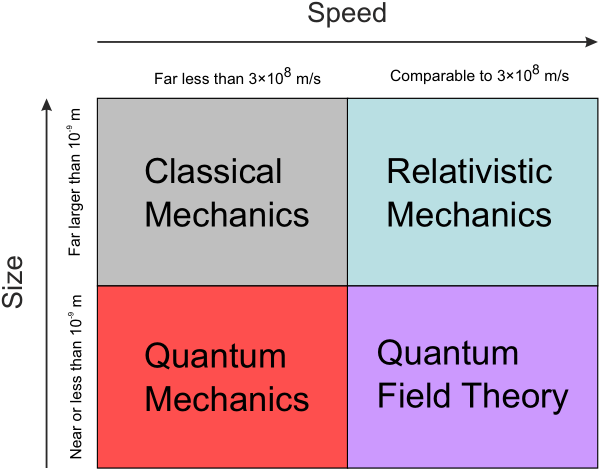
\includegraphics{../fig/theories.png}
\caption{Some theories.}\label{fig:theories}
\end{figure}

\section{Conclusion and Outlook}\label{conclusion-and-outlook}

Relativistic mechanics is probably the best way to describe a new theory of gravitation.
The future will show whether there is any application of our theories.

\appendix

\section{Some maths}\label{some-maths}

\begin{equation} E = m\cdot c^2\,, \label{eq:emc2}\end{equation}

Because people love to see equations.

\section*{References}\label{references}
\addcontentsline{toc}{section}{References}

\hypertarget{refs}{}
\hypertarget{ref-Einstein1905}{}
Einstein, Albert. 1905. ``{[}On the Electrodynamics of Moving Bodies.'' \emph{Annalen Der Physik} 322 (10): 891--921. doi:\href{https://doi.org/10.1002/andp.19053221004}{10.1002/andp.19053221004}.

\hypertarget{ref-Newton1730}{}
Newton, Isaac. 1730. \emph{Opticks, or a Treatise of the Reflections, Refractions, Inflections and Colours of Light}. William Innys. \url{http://books.google.com/books?id=XXu4AkRVBBoC}.

%%% MARTIN
\subsection{Acknowledgements}
{\small We thank R. Penrose, who time-travelled to Isaac and Albert, and initiated communication.
Thanks also to the anonymous reviewer who greatly improved this manuscript.}
%%%
\end{document}
